\documentclass{article}

\usepackage{pgf}
\usepackage{enumitem}
\setlist[1]{itemsep=-2pt}
\usepackage{tikz}
\usepackage[utf8]{inputenc}
\usetikzlibrary{arrows,automata}
\usetikzlibrary{positioning}
\usepackage{lscape}
\usepackage[left=4cm,textheight=674pt]{geometry}


\tikzset{
    state/.style={
           rectangle,
           rounded corners,
           draw=black, very thick,
           minimum height=2em,
           inner sep=2pt,
           text centered,
           },
}

\begin{document}
\begin{landscape}
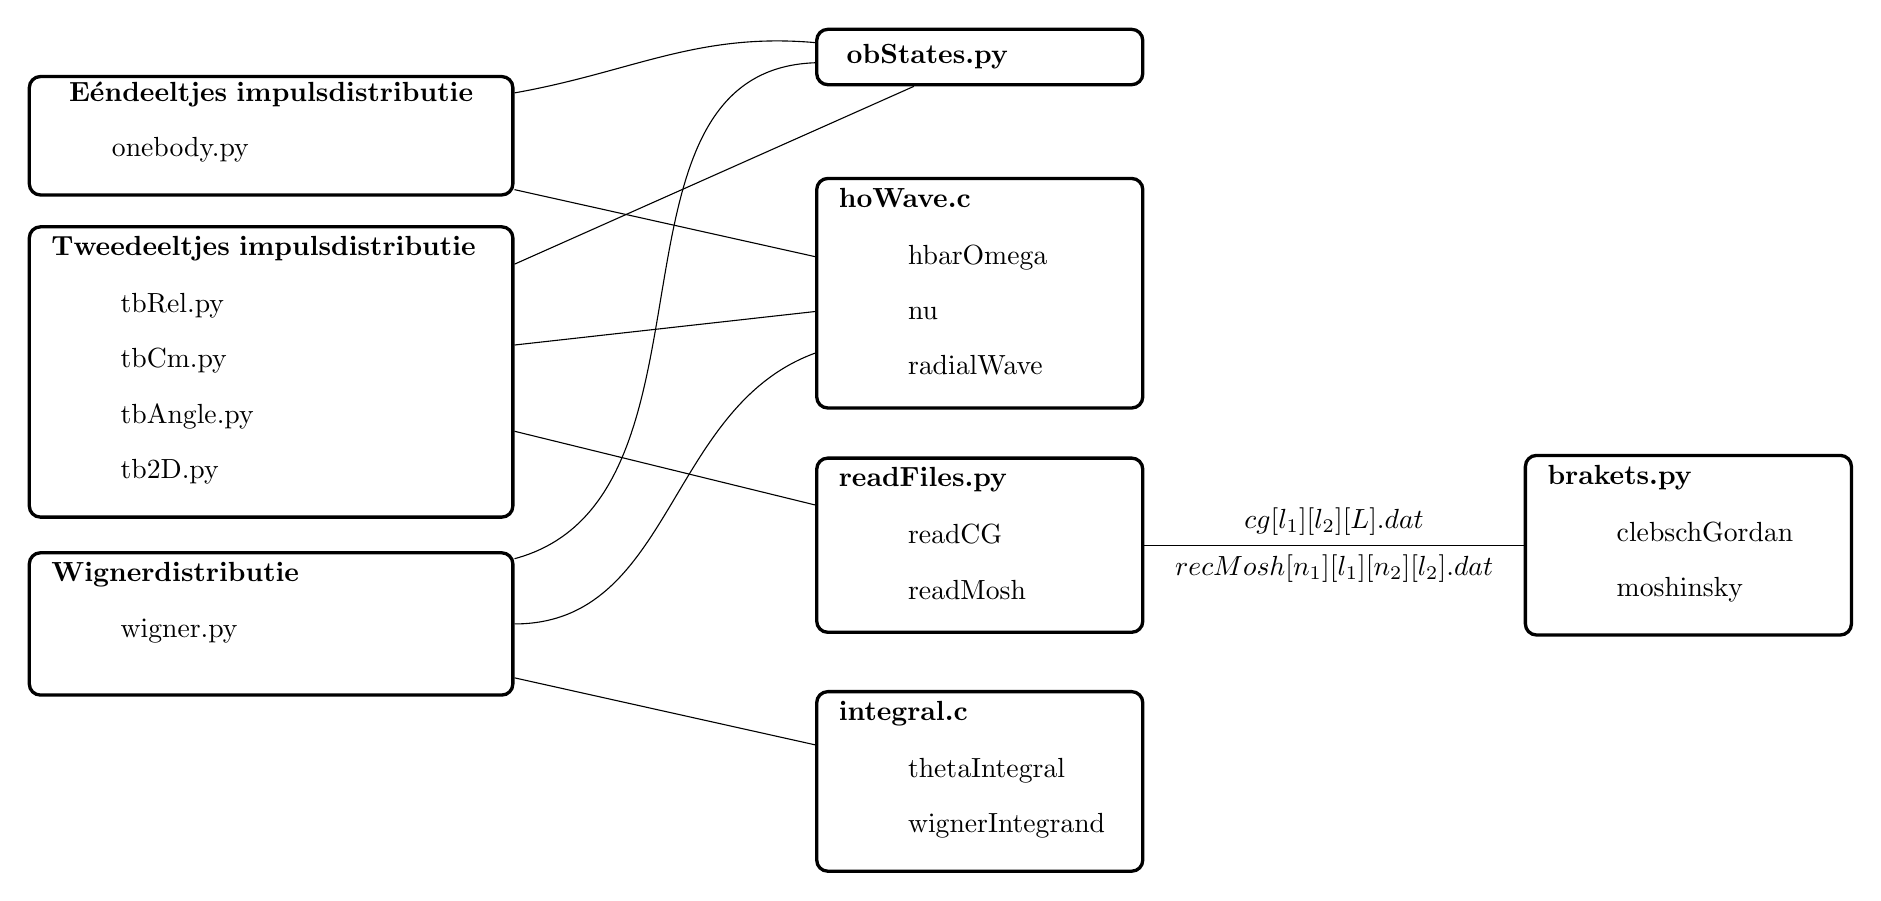
\begin{tikzpicture}[node distance= 2cm]

 % Position of onebody
 % Use previously defined 'state' as layout (see above)
 % use tabular for content to get columns/rows
 % parbox to limit width of the listing
 \node[state,text width=6cm,xshift=-4cm,] (ONEBODY) 
 {
  \textbf{E\'{e}ndeeltjes impulsdistributie}\\
  \parbox{5.8cm}{\begin{itemize}
  \item[] onebody.py
  \end{itemize}
  }\\[1em]
};
  
 % State: OBSTATES
 \node[state,    	% layout (defined above)
  text width=4cm, 	% max text width
  yshift=1cm, 		% move 2cm in y
  right of=ONEBODY, 	% Position is to the right of ONEBODY
  node distance=9cm, 	% distance to ONEBODY
  anchor=center] (OBSTATES) 	% posistion relative to the center of the 'box'
 {\parbox{3.8cm}{
 \begin{tabular} {l}	% content
  \textbf{obStates.py}\\
 \end{tabular}
 }};
 
 % STATE HOWAVE
 \node[state,
  below of=OBSTATES,
  yshift=-1cm,
  anchor=center,
  text width=4cm] (HOWAVE) 
 {%
 \begin{tabular}{l}
  \textbf{hoWave.c}\\
  \parbox{3.8cm}{
  \begin{itemize}
  	\item[] hbarOmega
  	\item[] nu
  	\item[] radialWave
 \end{itemize}   }\\[2em]
 \end{tabular}
 };
 
 
  % STATE READFILES
 \node[state,
  below of=HOWAVE,
  yshift=-1.2cm,
  anchor=center,
  text width=4cm] (READFILES) 
 {%
 \begin{tabular}{l}
  \textbf{readFiles.py}\\
  \parbox{3.8cm}{
  \begin{itemize}
  	\item[] readCG
  	\item[] readMosh
  \end{itemize}   }\\[1.5em]
 \end{tabular}
 };
 
  
  % STATE BRAKETS
 \node[state,
  anchor=center,
  right of=READFILES,
  node distance=9cm, 	
  text width=4cm] (BRAKETS) 
 {%
 \begin{tabular}{l}
  \textbf{brakets.py}\\
  \parbox{3.8cm}{
  \begin{itemize}
  	\item[] clebschGordan
  	\item[] moshinsky
  \end{itemize}   }\\[1.5em]
 \end{tabular}
 };
 
 
  % STATE INTEGRAL
 \node[state,
  below of=READFILES,
  yshift=-1.0cm,
  anchor=center,
  text width=4cm] (INTEGRAL) 
 {%
 \begin{tabular}{l}
  \textbf{integral.c}\\
  \parbox{3.8cm}{
  \begin{itemize}
  	\item[] thetaIntegral
  	\item[] wignerIntegrand
  \end{itemize}   }\\[1.5em]
 \end{tabular}
 }; 
 % STATE TWOBODY
 \node[state,
  below of=ONEBODY,
  yshift=-1cm,
  anchor=center,
  text width=6cm] (TWOBODY) 
 {%
 \begin{tabular}{l}
  \textbf{Tweedeeltjes impulsdistributie}\\
  \parbox{5.8cm}{
  \begin{itemize}
  	\item[] tbRel.py
  	\item[] tbCm.py
  	\item[] tbAngle.py
  	\item[] tb2D.py
  \end{itemize}   }\\[1.5em]
 \end{tabular}
 }; 
 
 % STATE WIGNER
 \node[state,
  below of=TWOBODY,
  yshift=-1.2cm,
  anchor=center,
  text width=6cm] (WIGNER) 
 {%
 \begin{tabular}{l}
  \textbf{Wignerdistributie} \\
  \parbox{5.8cm}{
  \begin{itemize}
  	\item[] wigner.py
  \end{itemize}   }\\[1.5em]
 \end{tabular}
 }; 

\draw (OBSTATES) 	to[in=10,out=175]  (ONEBODY) ;
\path (HOWAVE) 	edge (ONEBODY);
\path (OBSTATES) 	edge (TWOBODY) ;
\path (HOWAVE) 	edge (TWOBODY);
\draw (HOWAVE) 	to[in=0,out=200] (WIGNER);
\draw (OBSTATES) to[in=15,out=182]  (WIGNER);
\path (INTEGRAL) 	edge (WIGNER);
\path (BRAKETS) 	edge node[anchor=south,above]{$cg[l_1][l_2][L].dat$} node[anchor=north,below]{$recMosh[n_1][l_1][n_2][l_2].dat$}  (READFILES);
\path (READFILES) 	edge (TWOBODY);

\end{tikzpicture}

\end{landscape}

\end{document}